\renewcommand\thesection{\Roman{section}}

\section{In the main idea, it is not clear the sampling proportion between the data from known and unknown classes. How does this proportion affect the subsequent training?}
\label{Question: class number}
\subsection*{\underline{\textbf{Response:}}}

Thanks for your comments.
Without label information in the target domain, the sampling proportion between the data from known and unknown classes is not given in practice. 
During training, the proposed ThDAN is set to randomly sample data from the known and unknown classes.
Nevertheless, ThDAN can be trained under different sampling proportions.
To evaluate how the sampling proportion between the data from known and unknown classes could affect the performance, results of different numbers of training samples from unknown class are reported in Section \textit{5.3.4}.
\begin{figure*}[htb]
    \centering
    \subfloat[\footnotesize Accury \textit{w.r.t.} number of classes that are treated as the unknown]{
        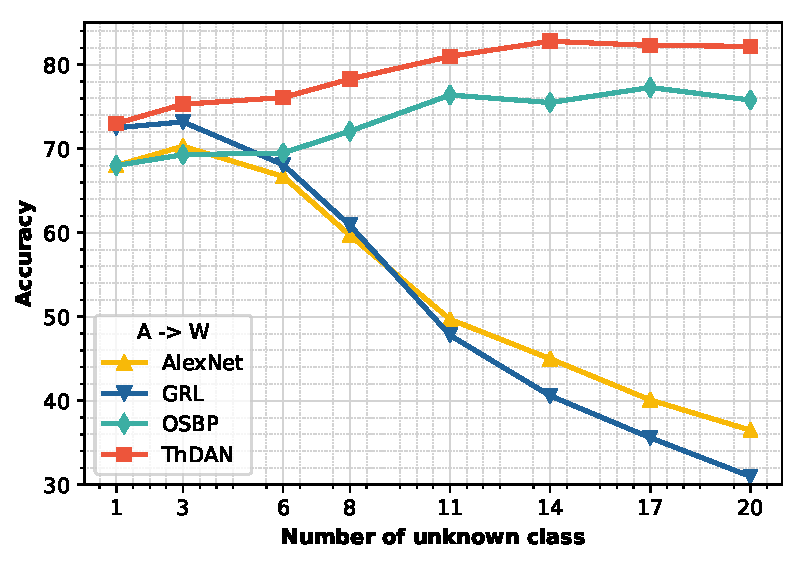
\includegraphics[width=0.33\textwidth]{contents/figures/pdf/analysis/class_change.pdf} 
        \label{figure: number of unknown class f}
    }
    \subfloat[\footnotesize Accury \textit{w.r.t.} ratio of used unknown samples]{
        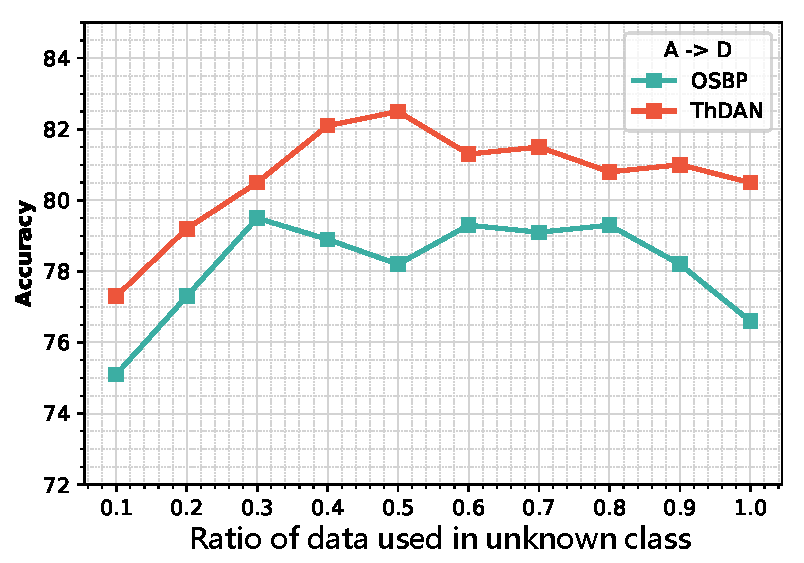
\includegraphics[width=0.34\textwidth]{contents/figures/pdf/analysis/nuknown_change.pdf} 
        \label{figure: ration of unknown f}
    } 
    \\
    \caption{
        (\textbf{a}): 
        The accuracy when we change the ratio of unknown samples in the adaptation task \textit{A$\to$D}. 
        (\textbf{b}): 
        The accuracy when we change the number of classes that are treated as the unknown in the adaptation task \textit{A$\to$W}. 
    }
    \label{figure: analysis change ratio}
\end{figure*}

All experiments are conducted on Office31 that contains 31 different classes.
In \figurename{\ref{figure: number of unknown class f}}, the first 10 classes are used as the known classes.
By increasing the number of classes that are treated as the unknown, the sampling proportion for data from the unknown class increases.
It is worth noting that the methods for close set domain adaptation will incur severe performance degradations.
This is because these methods can neither alleviate the negative transfer brought by the unknown class, nor effectively identify samples from the unknown class.
On the contrary, the methods proposed for open set domain adaptation will gain performance improvements by correctly rejecting samples from the unknown class.
However, threating too many classes as the unknown will deteriorate the knowledge transfer for the classification task.
Therefore the accuracy tends to decay at the end.

In \figurename{\ref{figure: ration of unknown f}}, we use the same 10 classes as the known classes and the rest as the unknown class.
To change the sampling proportion between the data from the known and unknown classes, we vary the ratio of data used in unknown class.
Specifically, value \textbf{0.1} of such ratio means that for each class that is treated as the unknown, only one-tenth data are used to train model. 
So reducing the ratio of data used in the unknown class will decrease the sampling proportion for data from the unknown class.
In this case, the models can hardly identify samples of the unknown class due to the lack of training data.
On the other hand, when this ratio is high, the negative effect of the unknown class will substantially increase.
This leads to performance degeneration of categorizing the known classes.

The experiments show that the sampling proportion between the data from known and unknown classes can substantially affect model performance for both the known and unknown classes.
Sampling too much data from the unknown class will degrade the performance of categorizing known classes.
On the other hand, sampling too little data from the unknown class will affect the performance of rejecting ``unknown''.

\section{From their reported results in \textcolor{blue}{Fig.7}, the adjust threshold of $\gamma_0$ is not sensitive to the accuracy of training, it is a bit strange.
Authors are encouraged to carefully check their claims by using more detailed reasons or more diverse data sets. }
\label{Question: threshold}
\subsection*{\underline{\textbf{Response:}}}

Thanks for your suggestions.
We have checked that the results reported in \textcolor{blue}{Fig.7c} are correct.
In the revised manuscript, we give more detailed analysis to illustrate that the adjust threshold of $\gamma_0$ is not sensitive to the accuracy of training.

\textcolor{blue}{Fig.7c} of the original manuscript is presented as follows,
\begin{figure}[htb]
    \centering
    \subfloat[Accury \textit{w.r.t.} the value of $\gamma_0$]{
        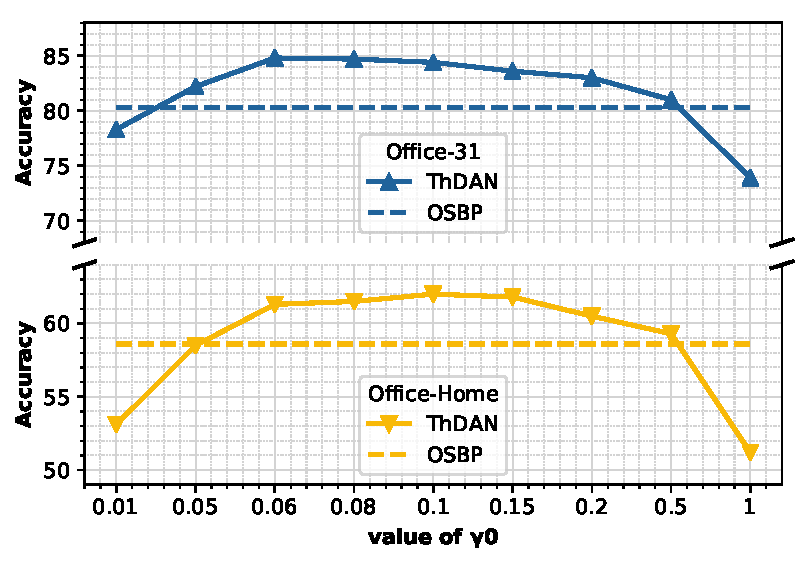
\includegraphics[width=0.33\textwidth]{contents/figures/pdf/analysis/sigma_change.pdf} 
        \label{figure: analysis in question 2}
    }
    \\
    \caption{
        The prediction accuracy of our method when we change the value of $\gamma_0$ on dataset Office-31 and Office-Home. 
    }
\end{figure}
\newline
\figurename{\ref{figure: analysis in question 2}} demonstrates the average accuracy of \textbf{6 tasks on Office-31} and \textbf{12 tasks on Office-Home} when $\gamma_0$ changes.
Compared with the baseline model OSBP, the proposed ThDAN can deliver considerable results on both Office-31 and Office-Home datasets in a wide range of $\gamma_0$.

To select transferable samples from target domain for domain adversarial training \cite{DomainAdversrialNetwork,ADDA,OpensetDA-bp}, a transferability threshold is adaptively computed during training:
\begin{equation}
    \label{eq: transferability thresholded}
    \beta(X_s, \gamma) = \mathbb{E}_{x \in X_s} w(x) - \gamma.
\end{equation}
The threshold $\beta$ is calculated by averaging the transferability score of a batch of source samples and a predefined $\gamma$.
In the training phase, we dynamically increase $\gamma$ from $0$ to $\gamma_0$ so that more samples of known classes can be selected.
Formally, $\gamma$ changes as follows,
\begin{equation}
    \label{eq: dynamic tolerable range}
    \begin{split}
        \gamma(n) &=
        \begin{cases}
            0 & ,\: n \in N_1 \\
            \gamma_0 \times  \sigma(n) & ,\: n\in N_2 \\
        \end{cases}.
    \end{split}
\end{equation}
Here $\sigma$ is a \textit{monotonically increasing function} with an upper bound of $1$.

To promote model convergence, we adopt the formula as \cite{DomainAdversrialNetwork} to reduce learning rate during training.
As a result, the transferable samples that are selected in the early stage would ``dominate'' the model training.
These samples engage in training sooner, so the gradient they produce can update the model with a larger learning rate.
As $\gamma$ approaches $\gamma_0$, the learning rate is relatively low, and the previously selected samples are likely to be selected again.
Therefore the newcomers have little impact on the model performance.
This directly reflects the insensitivity of value of $\gamma_0$ to classification accuracy.

The above explanation has been added in the revised manuscript.
Please refer to Section \textit{5.3.6} of the revised manuscript for details.

\renewcommand\thesection{\arabic{section}}
\setcounter{section}{0}

\section{The abstract needs to be redesigned.
    Open set domain adaptation (OSDA) should be a scenario.
    Authors claim to solve the OSDA problem. What is the problem?? This is unclear.
    It seems the author should firstly explain the OSDA setting and then present which issue they want to address. The first sentence of the abstract is a bit far away from their focus.
    More seriously, the introduction don not connect the abstract.
    For example, the beginning of the abstract explains the unsupervised domain adaptation, but the beginning of the introduction suddenly use deep learning to start this paper without unsupervised domain adaptation.
    Authors are encouraged to carefully reorganize their work, where the introduction must connect the abstract tightly.
    One sentence in the abstract should connect one logic in the introduction section.}
\subsection*{\underline{\textbf{Response:}}}


Thanks for your comments, the suggestions are of great help to improve our work.
In the revised manuscript, we redesigned the \textbf{abstract} and \textbf{introduction} for tighter logical connections.

The \textbf{abstract} has being redesigned as follows,
\begin{siderules}
    \textit{
        \footnotesize
        In recent years, many unsupervised domain adaptation (UDA) methods have been proposed to tackle the domain shift problem.
        Most existing UDA methods are derived for Close Set Domain Adaptation (\textit{CSDA}) in which source and target domains are assumed to share the same label space.
        However, target domain may contain unknown class different from the known ones in the source domain in practice, i.e., Open Set Domain Adaptation (\textit{OSDA}).
        Due to the presence of unknown class, aligning the whole distribution of the source and target domain for OSDA as in the previous methods will lead to negative transfer.
        Existing methods developed for OSDA attempt to assign smaller weights to target samples of unknown class.
        Despite promising performance achieved by existing methods, the samples of the unknown class are still used for distribution alignment, which make the model suffer from the risk of negative transfer.
        Instead of reweighting, this paper presents a novel method namely Thresholded Domain Adversarial Network (\textit{ThDAN}), which progressively selects transferable target samples for distribution alignment.
        Based on the fact that samples from the known classes must be more transferable than target samples of the unknown one, we derive a criterion to quantify the transferability by constructing classifiers to categorize known classes and to discriminate unknown class.
        In ThDAN, an adaptive threshold is calculated by averaging transferability scores of source domain samples to select target samples for training.
        The threshold is tweaked progressively during the training process so that more and more target samples from the known classes can be correctly selected for adversarial training.
        Extensive experiments show that the proposed method outperforms state-of-the-art domain adaptation and open set recognition approaches on benchmarks.
    }
\end{siderules}

According to the redesigned abstract, we have modified the \textbf{introduction} to make it connect to the abstract tightly.
The following Table \ref{table: logical} shows the logical connection between each paragraph of the introduction and each sentence of the abstract.
% Please add the following required packages to your document preamble:
% \usepackage{multirow}

% \newcommand\iw{0.05}
% \newcommand\cw{0.05}
% \renewcommand\tabularxcolumn[1]{m{#1}}
\newcommand\emmax[1]{\textcolor{red}{\textbf{#1}}}
\newcommand\methodyear[1]{\textcolor{blue}{#1}}
\newcommand\Tstrut{\rule{0pt}{2.6ex}}
\newcommand\Bstrut{\rule[-0.9ex]{0pt}{0pt}}

\newcommand{\centeritem}[1]{\noindent\parbox[c]{\hsize}{\footnotesize \vspace*{1mm} #1 \vspace*{1mm}}}

\begin{table*}[htb]
    \renewcommand{\arraystretch}{1.3}
    \caption{ The logical connection between paragraphs of the introduction and sentences of the abstract. }
    \label{table: logical}
    \centering
    \small
    % >{\itshape
    \begin{tabularx}{0.95\textwidth}{c| >{\itshape}X}
        \toprule[0.8pt]
        \textbf{\small Paragraph of Introduction} & \multicolumn{1}{c}{\textbf{\small Sentence of Abstract}}                                                                                                                                                                                                                              \\
        \bottomrule[0.8pt]
        \# 1             & \centeritem{In recent years, many unsupervised domain adaptation (UDA) methods have been proposed to tackle the domain shift problem.}                                                                                                          \\
        \hline
        \# 2             & \centeritem{Most existing UDA methods are derived for Close Set Domain Adaptation (\textit{CSDA}) in which source and target domains are assumed to share the same label space.
            However, target domain may contain unknown class different from the known ones in the source domain in practice, i.e., Open Set Domain Adaptation (\textit{OSDA}).}                                                                                            \\
        \hline
        \# 3             & \centeritem{Existing methods developed for OSDA attempt to assign smaller weights to target samples of unknown class.
            Despite promising performance achieved by existing methods, the samples of the unknown class are still used for training, which make the model suffer from the risk of negative transfer.}                                                                     \\
        \hline
        \# 4             & \centeritem{Instead of reweighting, this paper presents a novel method namely Thresholded Domain Adversarial Network (\textit{ThDAN}), which progressively selects transferable target samples for distribution alignment. ......} \\
        \bottomrule[0.8pt]
    \end{tabularx}
\end{table*}




\section{What is ``transferable''? How to evaluate it? Any definition to support this term?}
\label{question: transferable}
\subsection*{\underline{\textbf{Response:}}}

Unfortunately, there is no formal definition or mathematical formula for ``transferable'' in domain adaptation.
Generally, the word ``transferable'' is used to describe features.
Here we quote from \cite{DeepAdaptationNetworks}:
\begin{quote}
    \textit{the transferable features are the features that generalize well to novel tasks for domain adaption}
\end{quote}
While the later work \cite{TransferableAttentionDA} uses ``transferable'' to describe samples that contribute to the transfer task of domain adaptation.

In the scenario of \textit{open set domain adaptation}, we consider the target samples from the known classes are transferable samples since they can boost the classification performance of the model.
On the contrary, the target samples from the unknown class are considered as untransferable samples, this is because aligning distribution with them will incur negative transfer.

The proposed method evaluates transferability from two perspectives:

\textbf{Target samples from the known classes are able to confuse $G_d$.}
Here $G_d$ is the domain discriminator that gives the probability of being target domain.
For a target sample, $z$ denotes the corresponding deep feature representation. 
If $G_d(z)$ approaches to $1$, then the sample has a high probability of coming from the unknown class.
That is because the unknown class is only included in the target domain and can be almost perfectly discriminated from the source samples.
On the other hand, if $G_d(z)$ approaches to $0$, then the sample is more likely from the classes shared by domains, \textit{i.e,} known classes.
So the transferable samples from target domain are able to confuse $G_d$ to label them as the source samples.
Therefore we define the transferability $w_d(x)$ as inversely related to $G_d(z)$,
\begin{align}
    w_d(x) &= 1-G_d(z). \label{eq: domain transferability}
\end{align}

\textbf{Target samples from the known classes can be categorized by $G_{c, known}$.}
Here $G_{c, known}$ is the classifier that gives the probability distribution of known classes.
Due to the overlapping in the marginal distributions across domains, target samples from the known classes could be categorized correctly by the classifier $G_{c, known}$ trained on the source samples.
This leads to low entropy (high transferability) for the samples from the known classes.
For the samples from the unknown class, because they cannot be classified into one of the $K$ known classes, the uncertainty of the prediction measured by the entropy is large.
Therefore the transferability $w_c(x)$ can be defined as inversely related to the \textit{normalized} classification entropy $H$,
\begin{align}
    w_c(x) &=1-H(G_{c,\; known}(z)). \label{eq: class transferability}
\end{align}

Since Eq.(\ref{eq: domain transferability}) and Eq.(\ref{eq: class transferability}) measure the transferability from two independent perspectives, we can unify the transferability criterions as,
\begin{equation}
    \label{eq: transferability}
    w(x)=1-G_d(z)\cdot H(G_{c,\; known}(z)).
\end{equation}
The experiments in Section \textit{5} show that the transferability criterion of Eq.(\ref{eq: transferability}) works well for the proposed model to select target samples from the known classes for domain adversarial training.

\section{In \textcolor{blue}{Fig.1}, it is unclear why (d) must outperform the other methods.}
\subsection*{\underline{\textbf{Response:}}}

Thanks for your comments.
As a matter of fact, \textcolor{blue}{Fig.1} is used to illustrate the general idea of the proposed method.
\textcolor{blue}{Fig.1} of the original manuscript is presented as follows,

\begin{figure}[H]
    \centering
    \subfloat{
        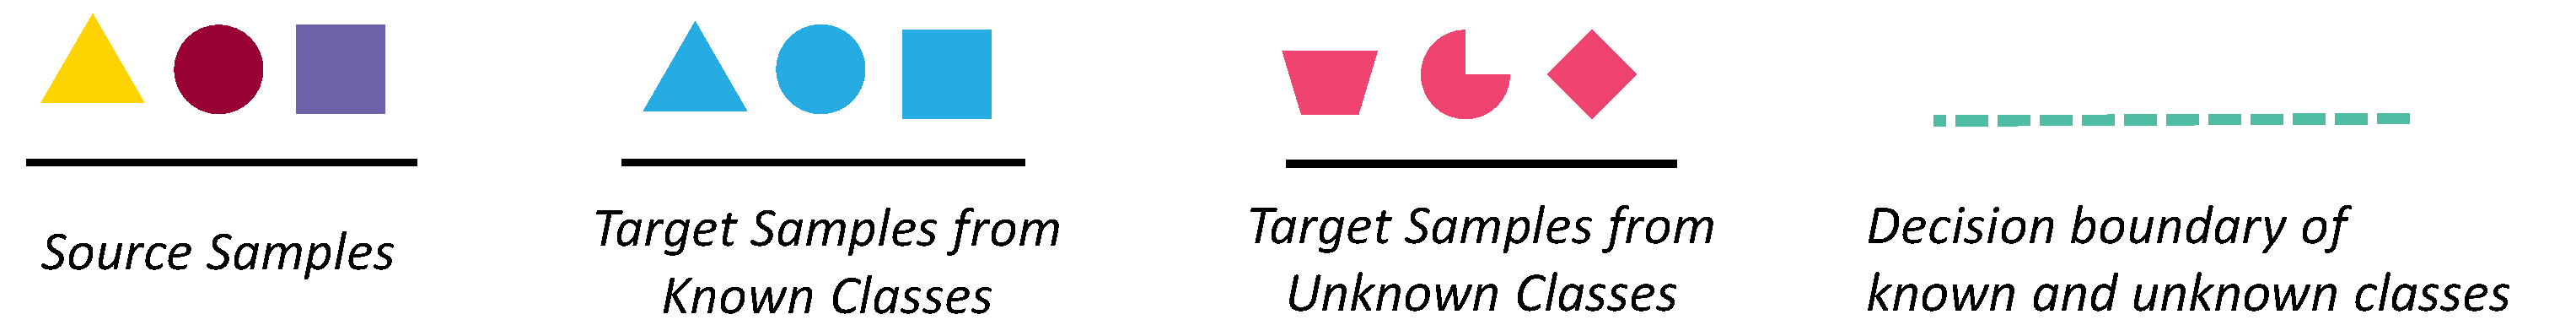
\includegraphics[width=0.55\textwidth]{contents/figures/pdf/overview/note.pdf} 
    }
    \\
    \addtocounter{subfigure}{-1}
    \subfloat[]{
        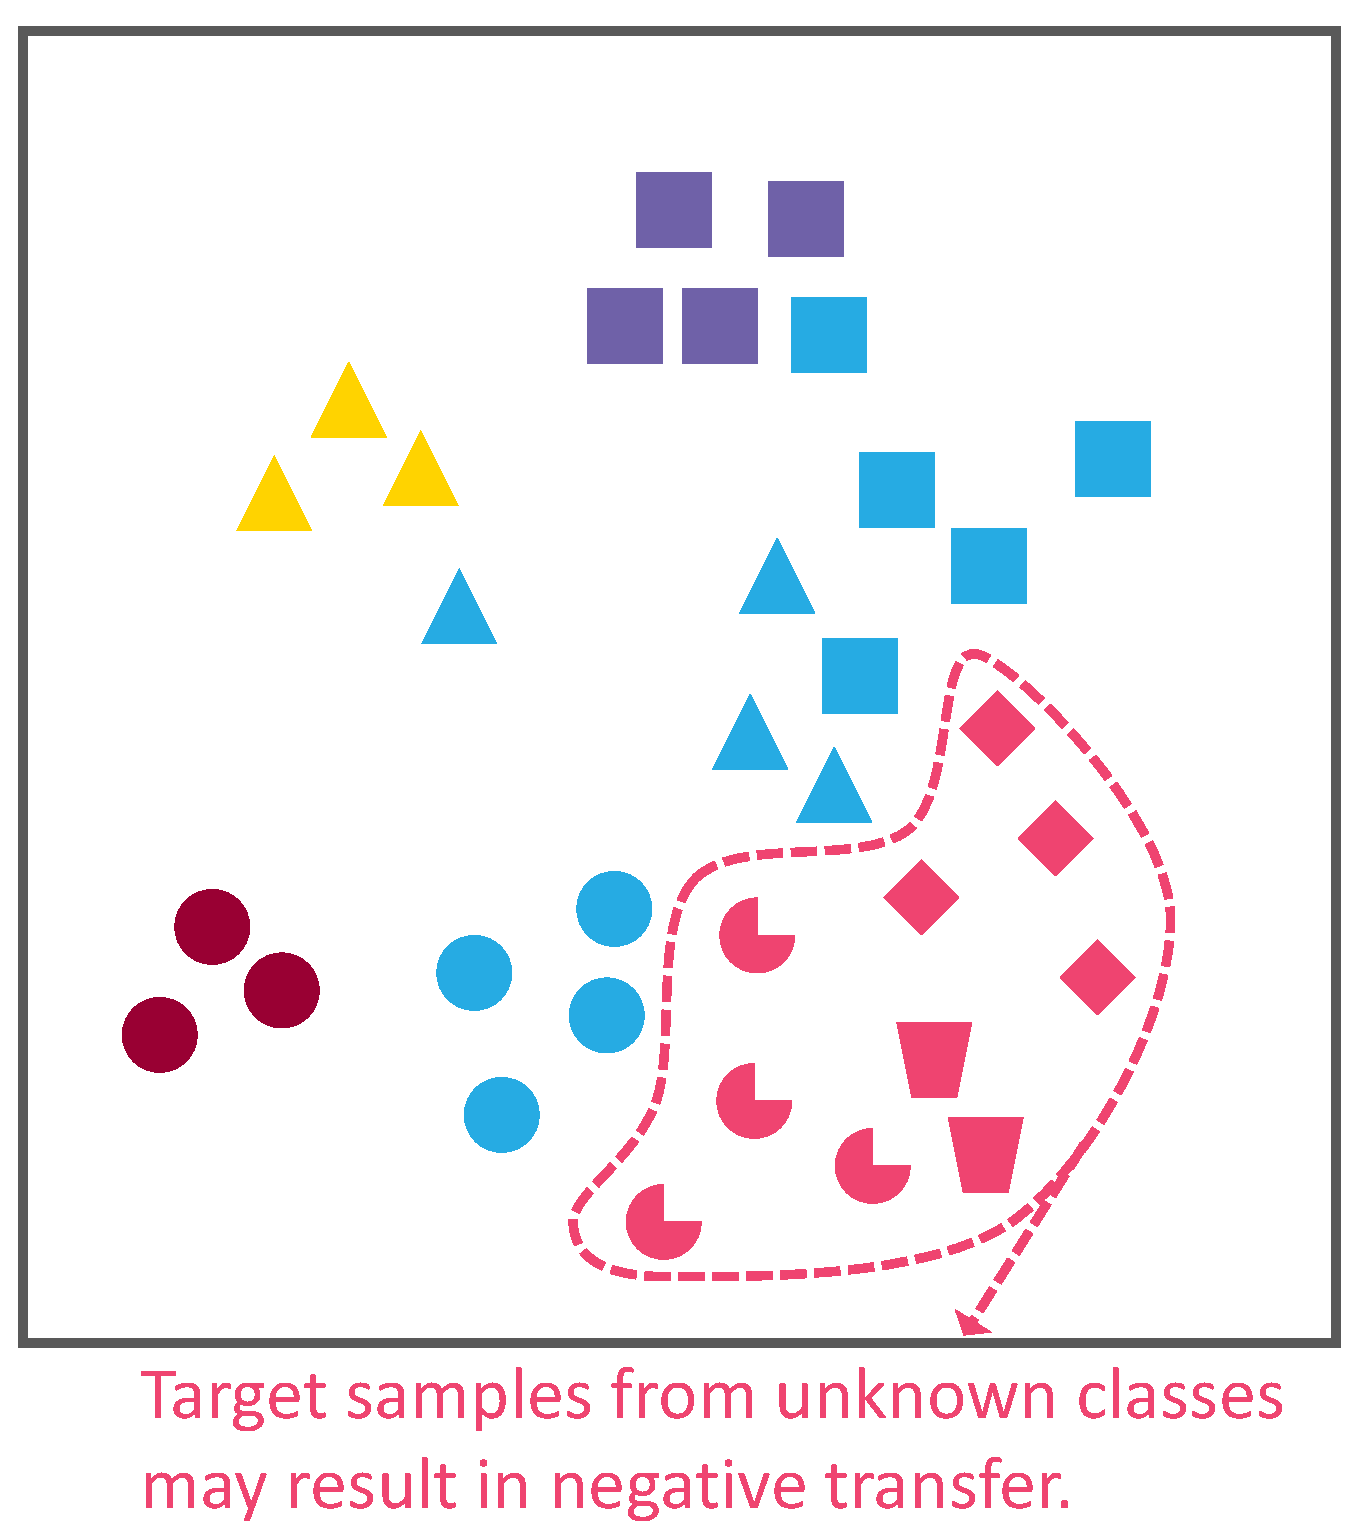
\includegraphics[width=0.22\textwidth]{contents/figures/pdf/overview/1.pdf} 
        \label{figure: reweighting based}
    } 
    \subfloat[]{
        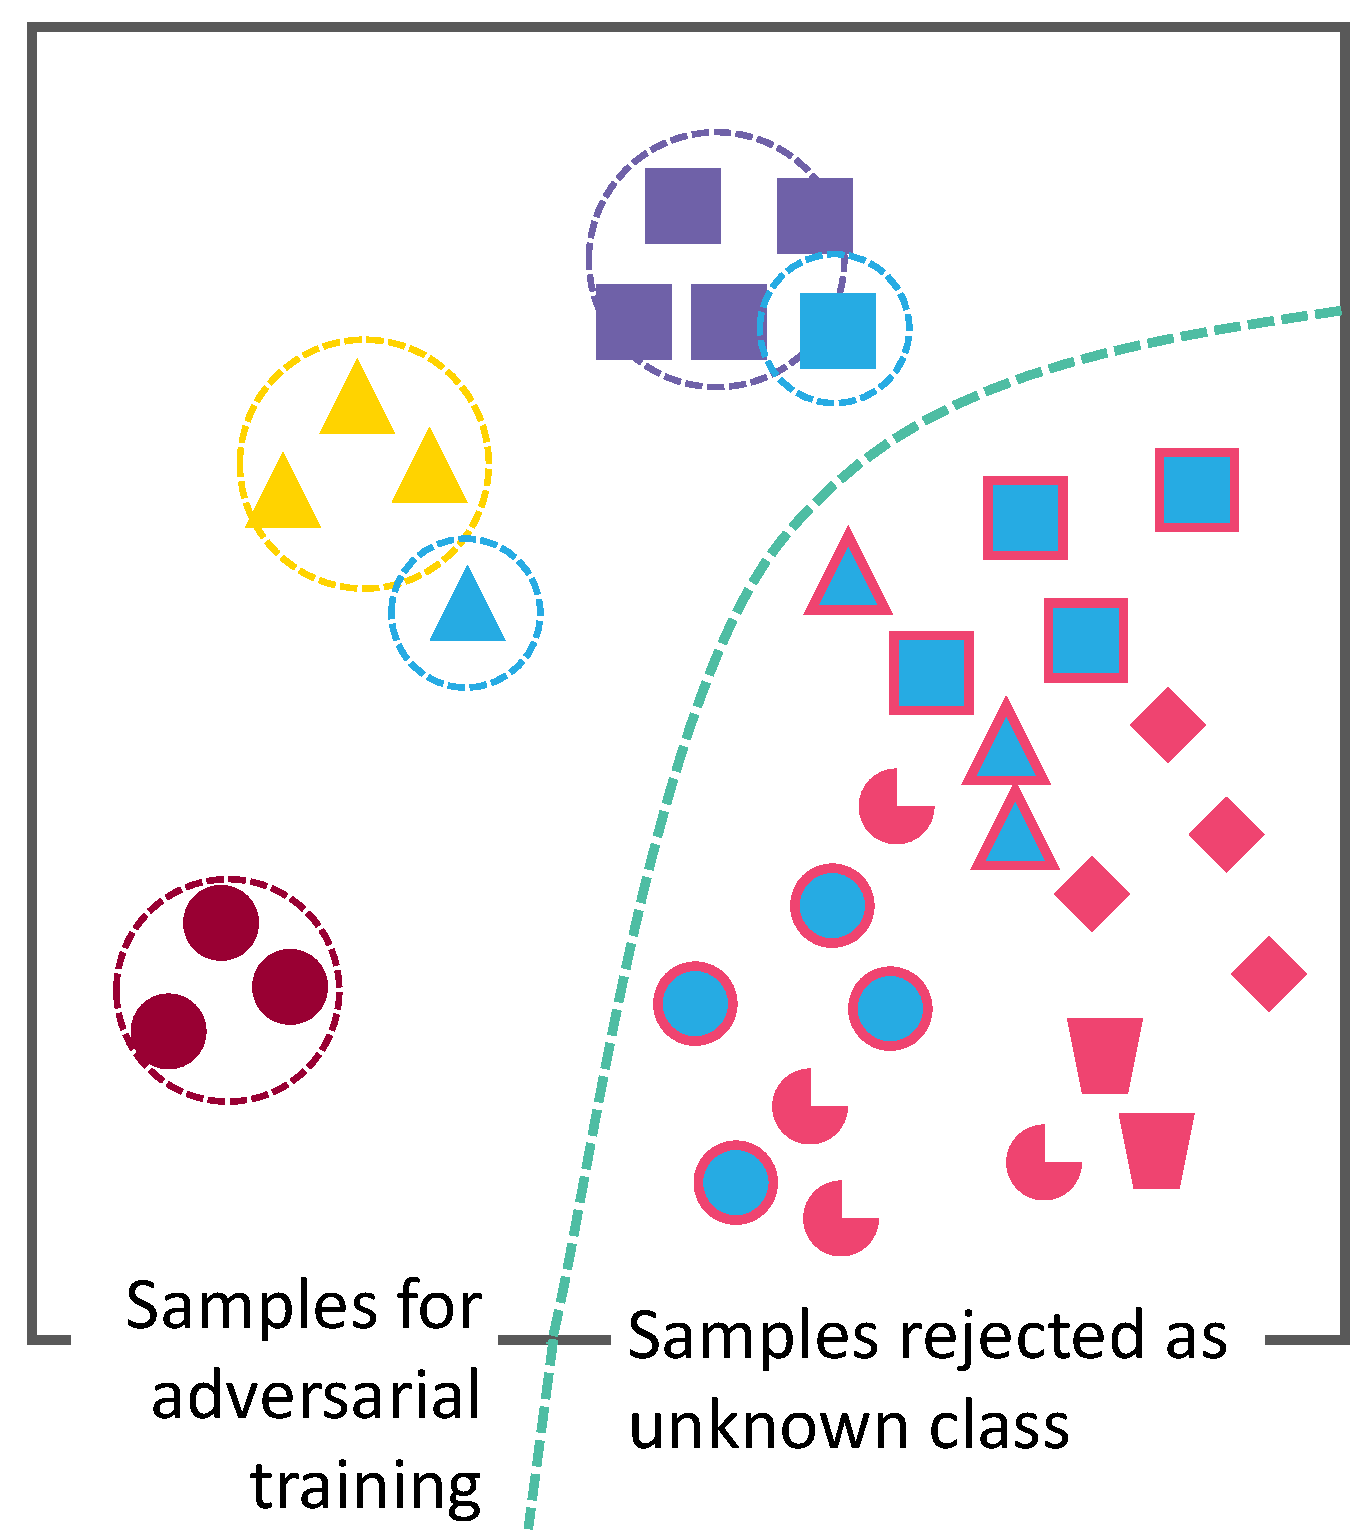
\includegraphics[width=0.22\textwidth]{contents/figures/pdf/overview/2.pdf} 
        \label{figure: ThDAN 1}
    } 
    \subfloat[]{
        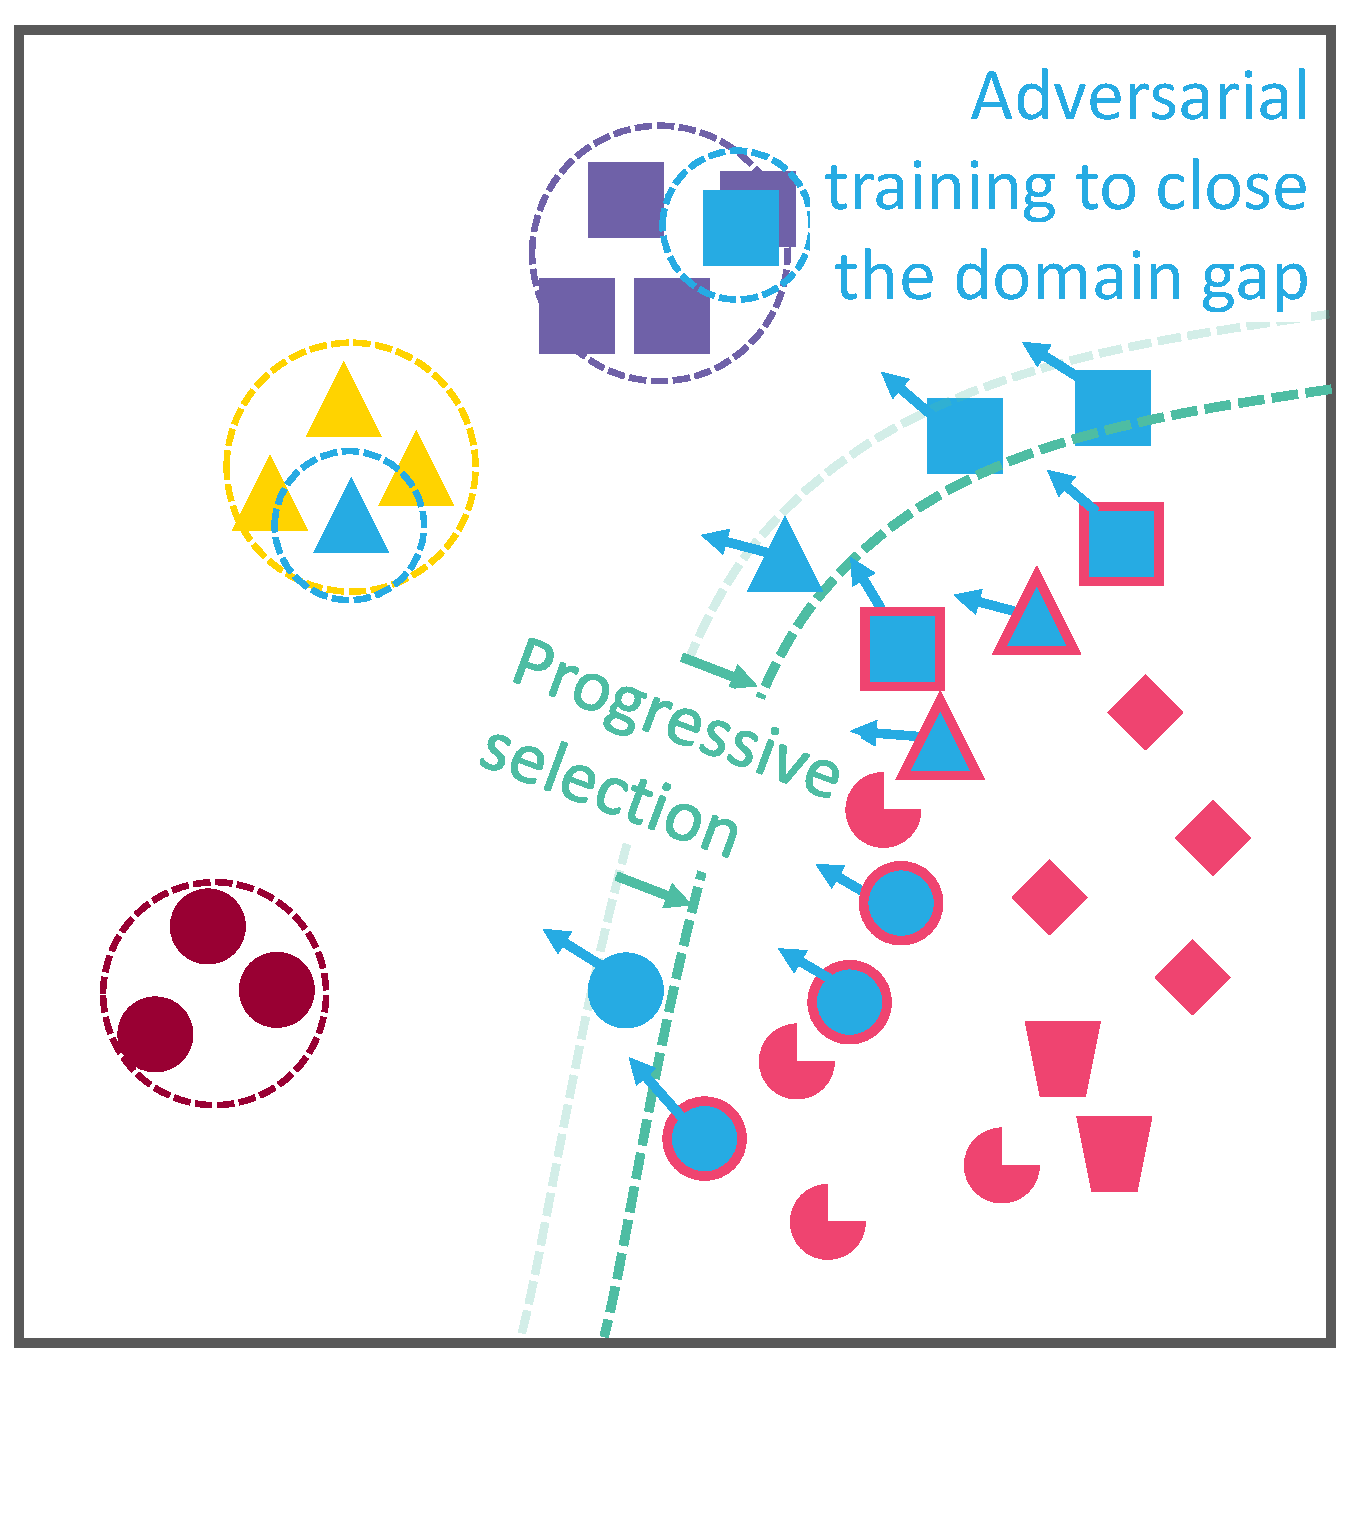
\includegraphics[width=0.22\textwidth]{contents/figures/pdf/overview/3.pdf} 
        \label{figure: ThDAN 2}
    } 
    % \hfil
    \subfloat[]{
        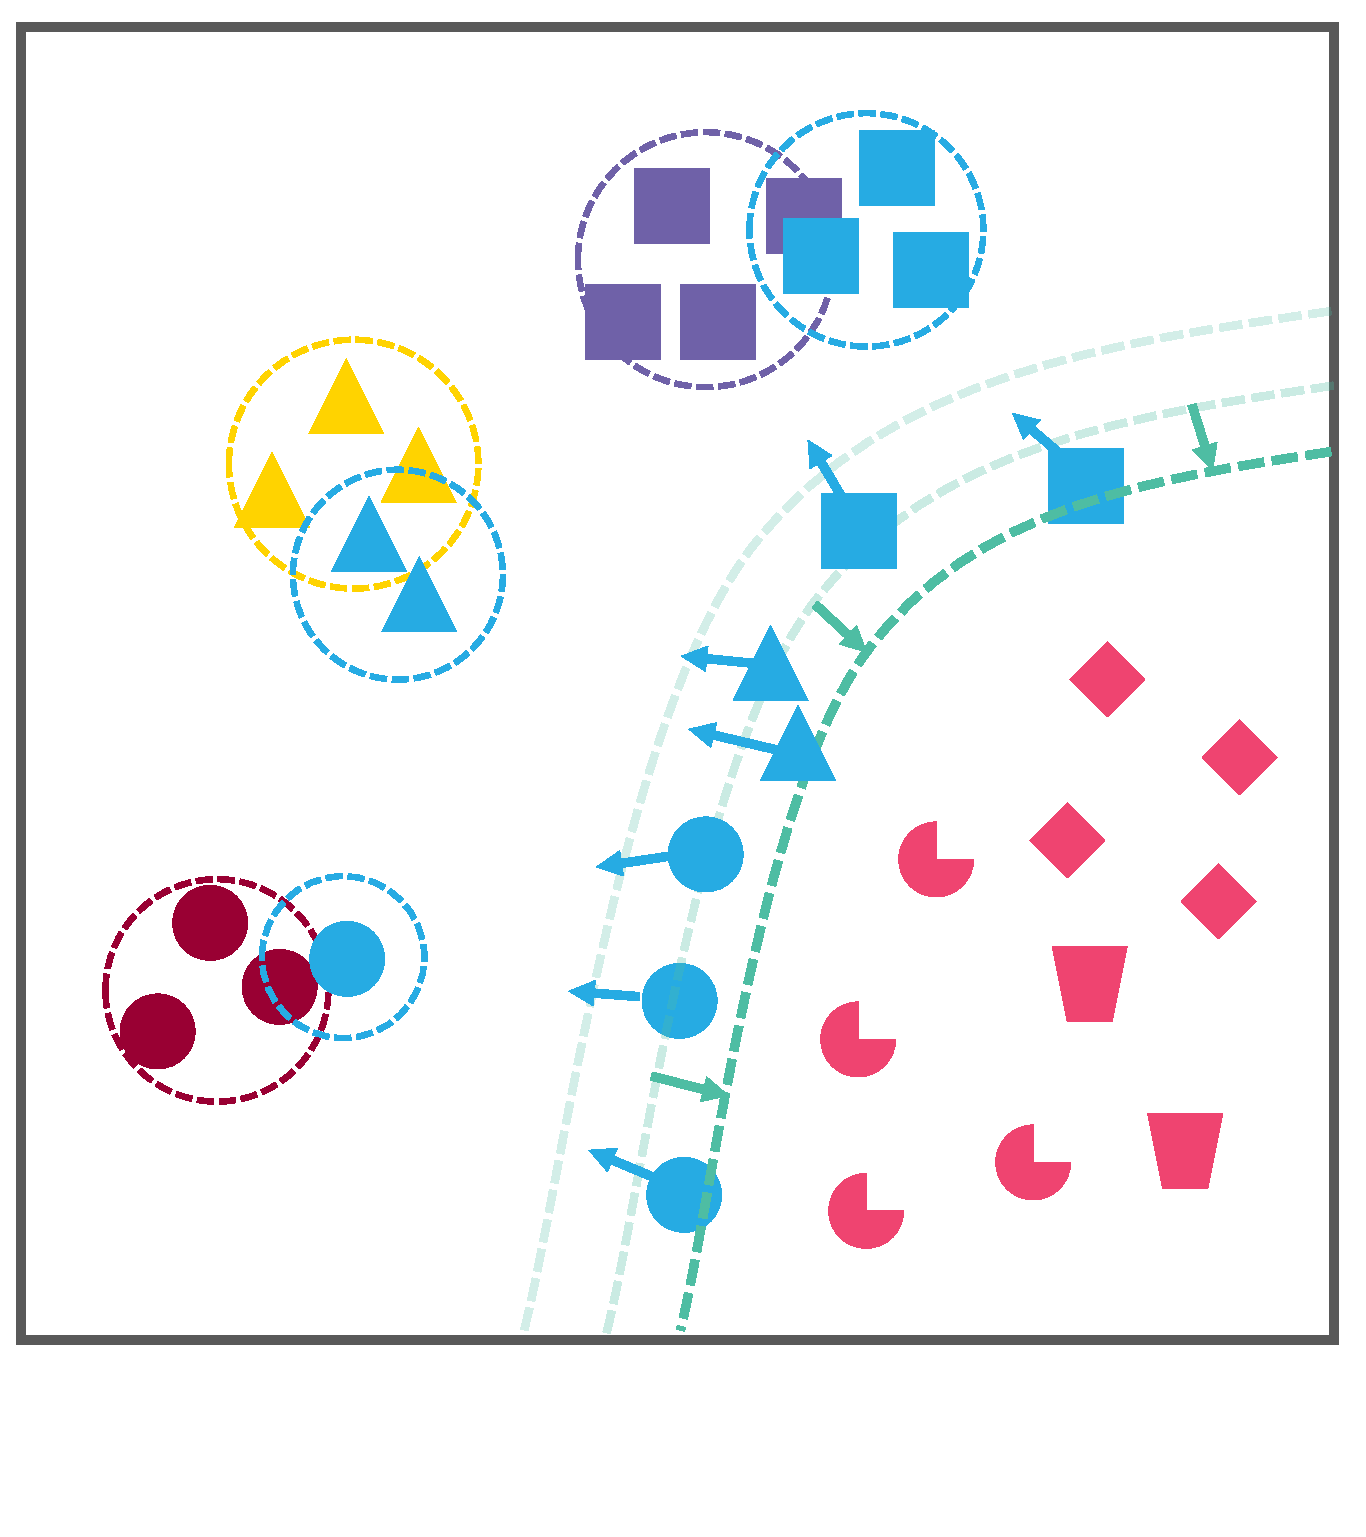
\includegraphics[width=0.22\textwidth]{contents/figures/pdf/overview/4.pdf} 
        \label{figure: ThDAN 3}
    }
    \caption{
        Figure1 of the original manuscript.
    } 
    \label{figure: overview} 
\end{figure}


% \newline
To make a clearer presentation for \figurename{\ref{figure: overview}}, we modify the caption in the revised manuscript as follows,
\begin{siderules}
    \textit{
        \footnotesize
        The general idea of the proposed Thresholded Domain Adversarial Network (\textit{\textbf{ThDAN}}).
        (\textbf{a}): Training samples for open set domain adaptation.
        (\textbf{b}): ThDAN builds a decision boundary of the transferability threshold to separate transferable and untransferable samples. 
        (\textbf{c}): To bridge the domain gap, the transferable samples from target domain are selected for domain adversarial training.
        Then ThDAN tweaks the transferability threshold to collect more target samples of known classes to enhance knowledge transfer.
        (\textbf{d}): More transferable target samples are selected for domain adversarial training. All the unselected target samples are rejected as ``unknown''.
    }
\end{siderules}


\section{What is ``domain-invariant features'' ?}
\subsection*{\underline{\textbf{Response:}}}

In domain-invariant feature space, the source and target domains have the same (or similar) marginal distributions, and the posterior distributions of the labels are the same across domains too \cite{DeepDomainConfusion}.
Hence, a classifier trained on the labeled source domain is likely to perform well on the target domain.

Specifically, the domain-invariant features can be obtained by \textit{domain adversarial training} \cite{DomainAdversrialNetwork,ADDA,OpensetDA-bp}.
The domain adversarial training is a minmax game: a domain discriminator is trained to separate the feature representation of the source domain from the one of the target domain, at the same time, feature generators are trained to deceive the domain discriminator.
In this work, we adopt the training scheme proposed in \cite{OpensetDA-bp} to enable the domain discriminator to identify samples of unknown class for open set domain adaptation.
Formally, the training procedure can be written as,
\begin{equation}
    \label{eq: training DANN}
    \begin{split}
        \min_{G_f^t} \max_{G_d} \mathscr{L}(G_d,G^{s}_{f},G_f^t) &=\mathbb{E}_{x\sim p_t(x)} \left[ \log \left(G_d\left(G_f^t\left(x\right)\right)\right) \right]\\
        &+\mathbb{E}_{x\sim p_s(x)}\left[ \log \left(1-G_d\left(G_f^s\left(x\right)\right)\right) \right].
    \end{split}
\end{equation}
$G_f^s$ and $G_f^t$ are the feature extractors for source and target samples, which share weights as in \cite{OpensetDA-bp}.
$G_d$ is a binary domain discriminator with all the source samples labelled as $0$ and all the target samples labelled as $1$.
By optimizing Eq.(\ref{eq: training DANN}) with fixed $G_d$, $G_f^t$ is confined to generate features that can not be discriminated by $G_d$ (\textit{i.e.} domain-invariant features).
Therefore the classifier $G_c$ that trained on the source domain can perform well for target samples.

\section{In the related work, CSDA does not have references.}
\subsection*{\underline{\textbf{Response:}}}
Thanks for your suggestion.
CSDA is referred to Close Set Domain Adaptation and we have added references \cite{ben2010theory,Elsevier-DeepVisualDA,TransferLearningSurvey} for the methods for CSDA in the revised manuscript.

\section{In section 2.1, "Another way to solve domain adaptation" is not suitable.
Domain adaptation is a setting in detailed ML tasks or a probability distribution issue.
Authors can obtain more information from S Ben-David's paper.}
\subsection*{\underline{\textbf{Response:}}}
Thanks for your comment.
We agree that the phrase ``Another way to solve domain adaptation'' is not precise.
This phrase is revised as ``Another approach for domain adaptation''.
Similar imprecise wordings have been modified in the revised manuscript.
Also, we have carefully read Ben-David's paper \cite{ben2010theory} to get a better understanding of domain adaptation and have cited this paper in the revised manuscript.


\section{Section 2.2 missed some new work from open-set domain adaptation.}
\subsection*{\underline{\textbf{Response:}}}
Thanks for your suggestions.
We add some new work \cite{PDA-fac,PDA-sep} of open set domain adaptation in Section \textit{2.2}, they are respectively from ICLR2019 and CVPR2019.

Furthermore, we implement \textit{Factorized Representations For Open Set Domain Adaptation \textbf{(FRFOSDA)}} model proposed in \cite{PDA-fac} in experiments on \textbf{Office-Hone} and \textbf{Office31} for comparisons.
Please refer to Section \textit{5} for more details.

\section{In Section 3, authors missed the definition on $C_t$. Is it the label space of target domain?}
\subsection*{\underline{\textbf{Response:}}}
Yes, $C_t$ is the label space of target domain.
In the revised manuscript, the definition on $C_t$ has been added in section \textit{3.1 open set domain adaptation} as follows,
\begin{siderules}
\small
$C_s$ and $C_t$ denote the label space of the source and target domain, respectively.
In the setting of open set domain adaptation, the label space of target domain contains the label space of source domain, \textit{i.e.}, $C_s \subset C_t$.
We refer to classes from $C_s$ as the known classes and classes from $C_t\backslash C_s$ as the unknown class.
\end{siderules}


\section{In Section 3.1, what is ``untransferable ones''?}
\subsection*{\underline{\textbf{Response:}}}

This question is related to Question \ref{question: transferable}.
In the setting of open set domain adaptation, the untransferable ones refer to the samples of unknown class in the target domain.
The proposed method selects untransferable samples by evaluating transferability as follows,
\begin{equation}
    \label{eq: split target examples untrnasferable}
    \begin{split}
        X_t^u=\{x|w(x) < \beta, x \in X_t \}.
    \end{split}
\end{equation}
Here $w$ is transferability calculator of Eq.(\ref{eq: transferability}).
To select untransferable samples, a transferability threshold $\beta$ is computed by Eq.(\ref{eq: transferability thresholded}).
Then samples from $X_t$ with transferability score $w(x)$ less than the threshold $\beta$ will be selected as untransferable samples, denoted as $X_t^u$.

\section{In \textcolor{blue}{Eq.(2)}, more strong reasons need to be presented to explain the $G_f$ and $G_d$. Why the use such settings to define them? Only based other's work?}
\subsection*{\underline{\textbf{Response:}}}

The reason why we use the setting ``$G_f$ and $G_d$ can be considered as the generative network and discriminate network of GAN respectively'' to define them in \textcolor{blue}{Eq.(2)} is that the domain adversarial training between $G_f$ and $G_d$ is similar to the training procedure of the original \textit{Generative Adversarial Nets (GAN)} \cite{goodfellow2014generative}.

In GAN, the \textit{discriminate network} $D$ and the \textit{generative network} $G$ are trained with the following objective,
\begin{equation}
    \label{eq: GAN}
    \begin{split}
        \min_G \max_D V(D,G) &= \mathbb{E}_{x\sim p_{data}(x)}[\log D(x)] \\ &+ \mathbb{E}_{z\sim p_z(z)}[\log (1-D(G(z)))].
    \end{split}
\end{equation}
In the learning framework of GAN, $D$ is trained to separate the feature representation of the true images and fake images, and $G$ is trained to generate fake images that can confuse $D$.
While in the domain adversarial training of Eq.(\ref{eq: training DANN}), $G_d$ is trained to separate the feature representation of the source domain from the target domain, and $G_f$ ($G_f^t$) is trained to generated target features that are able to confuse $G_d$.
The training procedure of $D$ and $G$ is very similar to the domain adversarial training of $G_d$ and $G_f$.
Therefore we can define $G_f$ and $G_d$ by the setting of GAN.

To better illustrate why \textcolor{blue}{Eq.(2)} gives the optimal $G_d$, we remove this phrase and add more formal proof in the revised manuscript.
Please refer to the reply to the next question for details.

\section{In the following, why does $G_d$ converge to the optimal?}
\subsection*{\underline{\textbf{Response:}}}

In the revised manuscript, \textcolor{blue}{Eq.(2)} is rewritten as:
\begin{equation}
    \label{eq: revised optimal}
    \begin{split}
        G_d^*(z) &= \frac{p_t(z)}{p_s(z)+p_t(z)}. \\
    \end{split}
\end{equation}
In \textcolor{blue}{Eq.(2)} of the original manuscript, the subscript of $z_t$ should be removed and $z$ is the deep feature representation of a sample, \textit{i.e.,} $z=G_f(x).$
The proof for the property that Eq.(\ref{eq: revised optimal}) gives the optimal $G_d$ with fixed $G_f^s$ and $G_f^t$ is shown as follows,
\begin{proof}
    For any $G_f^s$ and $G_f^t$, we train $G_d$ to maximize Eq.(\ref{eq: training DANN}):
    \begin{equation}
        \label{eq: proof optimal discriminator}
        \begin{split}
            \max_{G_d} \mathscr{L}(G_d,G^{s}_{f},G_f^t)  = &\int_x p_t(x)\log \left(G_d\left(G_f^t\left(x\right)\right)\right)
              + p_s(x) \log\left(1-G_d\left(G_f^s\left(x\right)\right)\right) \, dx
            \\ = &\int_z p_t(z)\log \left(G_d\left(z\right)\right)
              + p_s(z) \log\left(1-G_d\left(z\right)\right) \, dz.
        \end{split}
    \end{equation}
    We take the partial differential of the objective Eq.(\ref{eq: proof optimal discriminator}) with respect to $G_d$, and apply the Leibnizs rule to exchange the order of differentiation and integration to achieve optimal $G_d$ in $[0, 1]$ at Eq.(\ref{eq: revised optimal}).
\end{proof}

The proof has been added in Section \textit{3.2} of the revised manuscript.

\section{In \textcolor{blue}{Eq.(2)}, how to define $p_s$ and $p_t$?}
\subsection*{\underline{\textbf{Response:}}}

\textcolor{blue}{Eq.(2)} in the revised manuscript is as follows,
\begin{equation}
    \label{eq: revised optimal 1}
    \begin{split}
        G_d^*(z) &= \frac{p_t(z)}{p_s(z)+p_t(z)}. \\
    \end{split}
\end{equation}
Here $z$ is the deep feature representation of a sample, \textit{i.e.,} $z=G_f(x)$.
As stated in \textit{Section 3.1 open set domain adaptation} of the revised manuscript, $p_s (z)$ and $p_t (z)$ are probability distributions of feature representations in source and target domains respectively, as defined in \cite{PartialDA-iw}.

\section{In \textcolor{blue}{Eq.(9)}, what is  $X_t^k$?}
\subsection*{\underline{\textbf{Response:}}}

Thanks for your comments.
$X_t^k$ and $X_t^k$ denote the transferable and untransferable samples selected from a batch of target samples $X_t$, respectively.
\textcolor{blue}{Eq.(9)} of the original manuscript indicates such process,
\begin{equation}
    \label{eq: split target examples}
    \begin{split}
        X_t^k=\{x|w(x) \geq \beta, x \in X_t \}, \\
        X_t^u=\{x|w(x) < \beta, x \in X_t \}.
    \end{split}
\end{equation}
Here $w$ is the transferability calculator defined in Eq.(\ref{eq: transferability}).
In training, a transferability threshold $\beta$ is computed by Eq.(\ref{eq: transferability thresholded}) to split a batch of target training data $X_t$ into two parts, $X_t^k$ and $X_t^u$.
Specifically, $X_t^k$ denotes the transferable samples from the target domain, which will be selected for domain adversarial training, while $X_t^u$ denotes the untransferable ones that the model learns to identify as ``unknown''.

We add Section \textit{4.1} in the revised manuscript to clarify the proposed methods and equations, in which $X_t^k$ and $X_t^u$ are explained.

\section{A same controversial issue appears again: Sample selection is the key step for this model to address open set domain adaptation.}
\subsection*{\underline{\textbf{Response:}}}

Thanks for your reminding.
This sentence has been modified as ``The sample selection algorithm will substantially affect the performance of ThDAN for open set domain adaptation''.

Similar imprecise wordings have been modified in the revised manuscript.


\section{In the experiments, why do you use different setting to begin the experiments in Section 4.2.1? Authors are encouraged to explain the inherent reasons.}
\subsection*{\underline{\textbf{Response:}}}

Thanks for your suggestions.
To evaluate the efficacy of the threshold tweaking techniques proposed for ThDAN, ablation studies on Office-31, OfficeHome and VisDA datasets are reported in Section \textit{4.2.1}, \textit{4.2.2} and \textit{4.2.3}.
The ablation studies involve 3 kinds of ThDAN variants:
(\textbf{1}) \textit{\textbf{ThDAN-m-dy}} is the original setting that calculates the transferability threshold based on mini-batch samples and a fixed $\gamma$.
(\textbf{2}) \textit{\textbf{ThDAN-dy}} is the variant that applies exponential moving average to update the transferability threshold.
(\textbf{3}) \textit{\textbf{ThDAN}} further takes advantage of dynamic $\gamma$ to tweak the transferability threshold.

In order to better understand how the proposed method performs under ablation settings, we add Section \textit{5.3.1 Ablation Study} in the revised manuscript.
Please refer to the revised manuscript for details.


\section{A same issue appear again in the settings of Section 4.2.2.}
\subsection*{\underline{\textbf{Response:}}}

Thanks for your reminding.
The ablation analysis in the original \textcolor{blue}{Section 4.2.2} has been reorganized in Section \textit{5.3.1 Ablation Study} of the revised manuscript.


\section{The results analysis in Section 4.2.3 is unclear. More detailed reasons need to be present to support your conclusion.}
\subsection*{\underline{\textbf{Response:}}}

The results of \textcolor{blue}{Section 4.2.3} are presented as follows,
% Please add the following required packages to your document preamble:
% \usepackage{multirow}

% \newcommand\iw{0.05}
% \newcommand\cw{0.05}
% \renewcommand\tabularxcolumn[1]{m{#1}}
\newcommand\emmax[1]{\textcolor{red}{\textbf{#1}}}
\newcommand\methodyear[1]{\textcolor{blue}{#1}}
\newcommand\Tstrut{\rule{0pt}{2.6ex}}
\newcommand\Bstrut{\rule[-0.9ex]{0pt}{0pt}}

\begin{table*}[htb]
    \renewcommand{\arraystretch}{1.3}
    \caption{Accuracy (\%) of each method with 6 shared class on VisDA. }
    \label{table: exp on visDA}
    \centering
    \small
    \begin{tabularx}{0.95\textwidth}{r Y Y Y Y Y Y Y >{\itshape}Y >{\itshape}Y }
        \toprule[0.8pt]
        \multicolumn{1}{c}{\multirow{2}{*}{Method}} & \multicolumn{9}{c}{  class-wise accuracy on VisDA}                                                                       \\ \cmidrule[0.1pt]{2-10}
        \multicolumn{1}{c}{}                        & Bcycle                                             & Bus  & Car  & Mcycle & Train & Truck & Unkown & Avg.All & Avg.Known \\
        \hline
        OSVM  \methodyear{[ECCV, 2014]}                                      & 4.8                                                & 45.0 & 44.2 & 43.5   & 59.0  & 10.5  & 57.4   & 37.8    & 34.5      \\
        MMD  \methodyear{[NIPS, 2007]}                                  & 0.2                                                & 30.9 & 49.1 & 54.8   & 56.1  & 8.1   & 61.3   & 37.2    & 33.2      \\
        GRL  \methodyear{[JMLR, 2016]}                                   & 9.1                                                & 50.5 & 53.9 & 79.8   & 69.0  & 8.1   & 42.5   & 44.7    & 45.1      \\
        OSBP  \methodyear{[ECCV, 2018]}                                       & 48.0                                               & 67.4 & 39.2 & 80.2   & 69.4  & \emmax{24.9}  & 80.3   & 58.5    & 54.8      \\
        \hline
        ThDAN-dy                                    & 52.6                                               & 69.5 & 58.8 & 83.1   & 72.3  & 12.3  & 84.5   & 61.8    & 58.1      \\
        ThDAN                                 & \emmax{55.2}                                               & \emmax{70.8} & \emmax{61.4} & \emmax{85.6}   & \emmax{74.8}  & 10.0  & \emmax{88.8}   & \emmax{63.8}    & \emmax{59.6}      \\
        \bottomrule[0.8pt]
    \end{tabularx}
\end{table*}


To better support our conclusion on Table \ref{table: exp on visDA}, we modify the analysis as follows,
\begin{siderules}
    \small
    In the experiments on VisDA, the \textit{training} split is used as the source domain and the \textit{validation} one as the target domain.
    We choose 6 categories, i.e., bicycle, bus, car, motorcycle, train and truck as the known classes, and the other 6 categories as the unknown class.
    The classification results are shown in Table \ref{table: exp on visDA}, where \textit{Avg.All} and \textit{Avg.Known} indicate the accuracy averaged over all classes and the known classes, respectively.
    For the classification for known classes, the proposed ThDAN can exceed other methods in almost every class and in the average, which means our method can effectively transfer knowledge for the adaptation task.
    % Compared with OSBP model, which uses all target samples for domain adversarial training, the superiority of ThDAN is clear.
    This is because ThDAN better avoids the negative transfer by aligning distributions with target samples of high transferability.
    Also, ThDAN improves the discrimination accuracy for the unknown class by a big margin.
    This further verifies the efficiency of the sample selection algorithm, since ThDAN is trained to reject the unselected (or untransferable) samples as ``unknown''. 
\end{siderules}

\section{Please carefully check the claim in \textcolor{blue}{Fig.7}.}
\subsection*{\underline{\textbf{Response:}}}

Thanks for your reminding.
\textcolor{blue}{Fig.7} of the original manuscript is included as follows,
\begin{figure}[H]
    \centering
    \subfloat[\footnotesize Accury \textit{w.r.t.} ratio of used unknown samples]{
        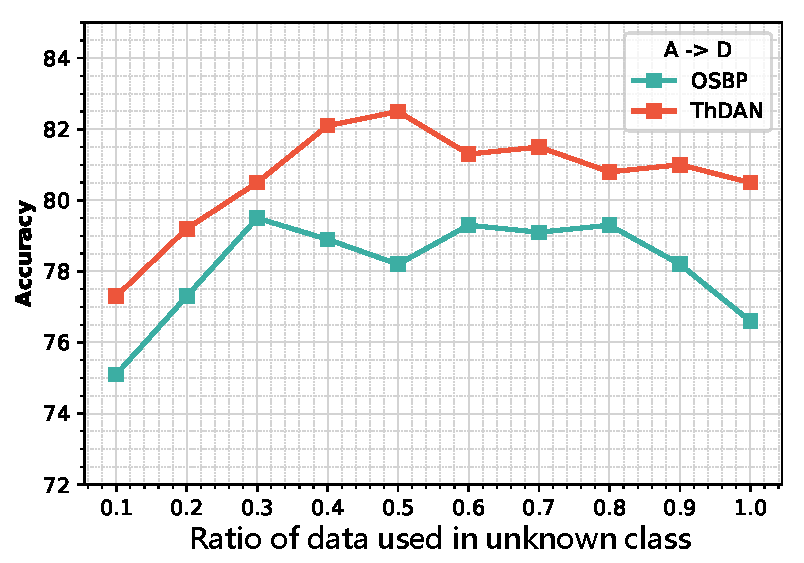
\includegraphics[width=0.34\textwidth]{contents/figures/pdf/analysis/nuknown_change.pdf} 
        \label{figure: ration of unknown}
    } 
    \subfloat[\footnotesize Accury \textit{w.r.t.} number of classes that are treated as the unknown]{
        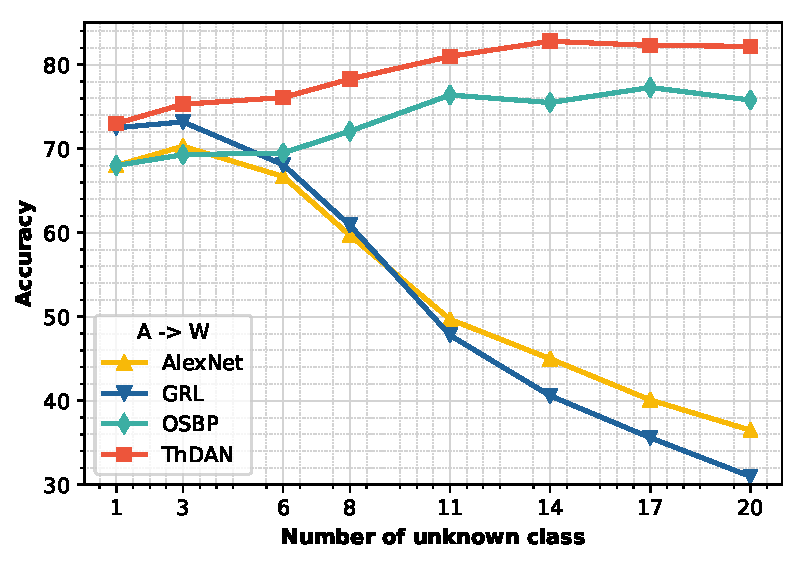
\includegraphics[width=0.33\textwidth]{contents/figures/pdf/analysis/class_change.pdf} 
        \label{figure: number of unknown class}
    }
    \subfloat[Accury \textit{w.r.t.} value of $\gamma_0$]{
        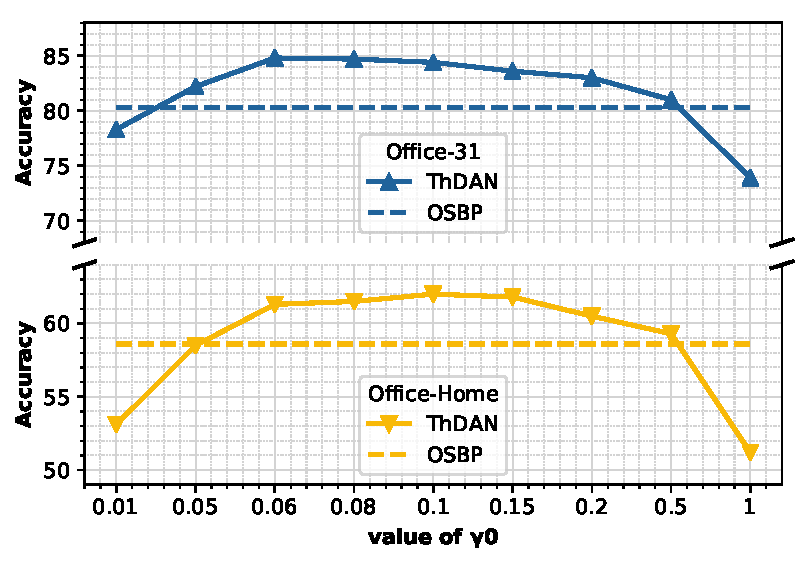
\includegraphics[width=0.33\textwidth]{contents/figures/pdf/analysis/sigma_change.pdf} 
        \label{figure: changing of sigma}
    }
    \\
    \caption{ }
    \label{figure: analysis}
\end{figure}

In the revised manuscript, the claims of \figurename{\ref{figure: analysis}} are modified for clearer representation.
The rewritten claims have been stated in the previous replies:
\begin{itemize}
    \item  In the response to \textbf{Question \ref{Question: class number}}, we modify the claims of \figurename{\ref{figure: ration of unknown}} and \figurename{\ref{figure: number of unknown class}} by adding more analysis to explain how the sampling proportion between the data from known and unknown classes could affect the performance.
    \item In the response to \textbf{Question \ref{Question: threshold}}, we modify the claims of \figurename{\ref{figure: changing of sigma}} by providing a more detailed analysis on why the proposed method is insensitive to the value of $\gamma_0$.
\end{itemize}

\section{Some equations missed ``,'' or ``.'' at their ends.}
\subsection*{\underline{\textbf{Response:}}}

Thanks for your reminding.
The equations in the revised manuscript have been corrected.


